\documentclass[12pt]{article}
\usepackage[T2A]{fontenc}
\usepackage[utf8]{inputenc}
\usepackage{multirow}
\usepackage{caption}
\usepackage{subcaption}
\usepackage{amsmath}
\usepackage{changepage}
\usepackage{graphicx}
\usepackage{float}
\usepackage[english,russian]{babel}
\usepackage{amsmath, amsfonts, amssymb, amsthm, mathtools}
\usepackage{xcolor}
\usepackage{array}
\usepackage{hyperref}
\usepackage[top = 1.5cm, left = 1.5 cm, right = 1.5 cm, bottom = 3 cm]{geometry}
\graphicspath{ {./images/} }
 
\title{Измерение коэффициента диффузии гелия при атмосферном давлении.}
\author{Шахматов Андрей, Б02-304}
\date{\today}
  
\begin{document}
\begin{titlepage}
    \begin{center}
        {\large МОСКОВСКИЙ ФИЗИКО-ТЕХНИЧЕСКИЙ ИНСТИТУТ (НАЦИОНАЛЬНЫЙ ИССЛЕДОВАТЕЛЬСКИЙ УНИВЕРСИТЕТ)}
    \end{center}
    \begin{center}
        {\large Физтех-школа физики и исследований им. Ландау}
    \end{center}
    
    
    \vspace{3cm}
    {\huge
        \begin{center}
            \textbf{Измерение коэффициента диффузии гелия при атмосферном давлении.}
        \end{center}
    }
    \vspace{2cm}
    \begin{flushright}
        {\LARGE Автор:\\ Шахматов Андрей Юрьевич \\
            \vspace{0.2cm}
            Б02-304}
    \end{flushright}
    \vspace{7 cm}
    \begin{center}
        Долгопрудный 2024
    \end{center}
\end{titlepage}

% \maketitle

\begin{abstract}
    Исследован метод получения высокого вакуума с использованием диффузионного насоса. Измерена 
    скорость откачки системы насосом а также скорость ухудшения вакуума из-за микротечей.       
\end{abstract}

\tableofcontents

\section{Введение}
Цель настоящей работы заключалась в исследовании получения вакуума с использованием ротационного 
форвакуумного насоса и диффузионного высоковакуумного насоса. 

\section{Методика}
\subsection*{Экспериментальная установка}
 В данной работе используются традиционные методы откачки механическим форвакуумным насосом до давления $10^{-2}$ торр и диффузионным масляным насосом до давления $10^{-4}$ торр. \\
 	Установка изготовлена из стекла,
 и состоит из форвакуумного баллона (ФБ), высоковакуумного диффузионного насоса (ВН), высоковакуумного баллона (ВБ), масляного (М) и ионизационного (И) манометров, термопарных манометров ($\text{М}_1$ и $\text{М}_2$), форвакуумного насоса (ФН) и соединительных кранов ($K_1, K_2,..., K_6$) (рис. 1). Кроме того, в состав установки входят: вариатор
 (автотрансформатор с регулируемым выходным напряжением), или
 реостат и амперметр для регулирования тока нагревателя диффузионного насоса. \\
  \begin{figure}[!h]
 	\centering
 	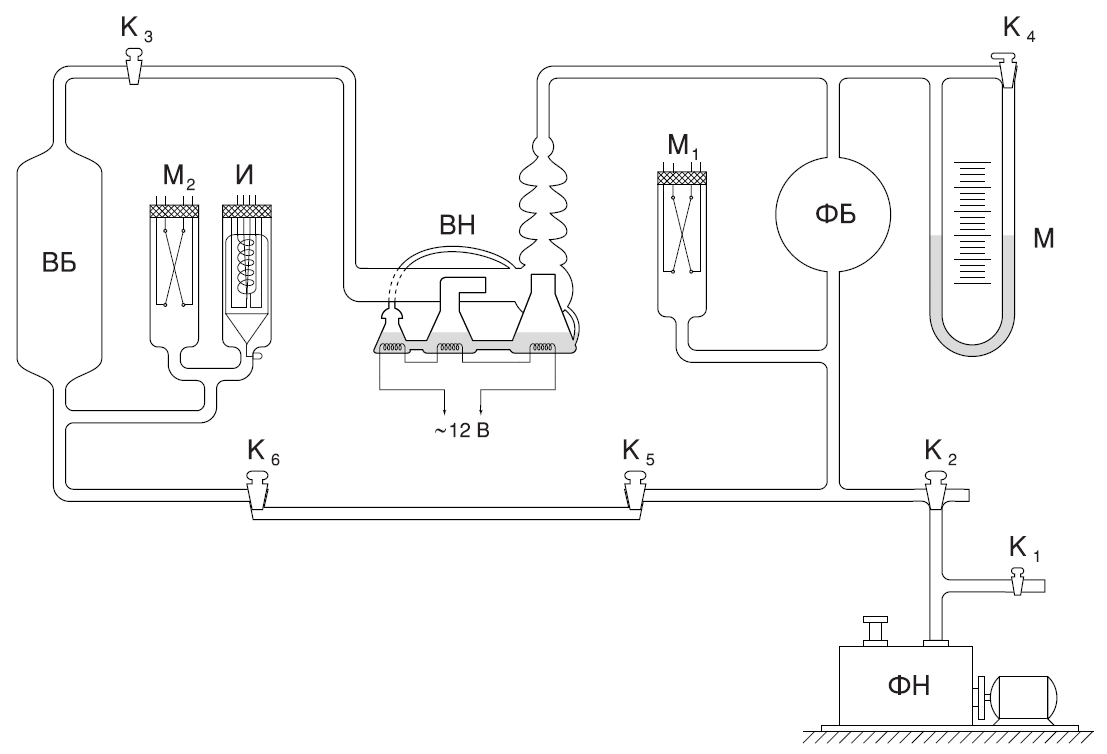
\includegraphics[width=0.5\linewidth]{Схема установки.PNG}
 	\caption[]{Схема установки}
 	\label{fig:Схема установки}
 \end{figure}
 Все краны вакуумной установки стеклянные. Стенки кранов тонкие, пробки кранов полые и составляют одно целое с рукоятками. Пробки кранов притерты к корпусам. Для герметизации используется вакуумная смазка. \\
 Устройство и принцип действия \textit{форвакуумного насоса} схематически, но довольно ясно изображены на рис 2. В положениях <<а>> и <<б>> пластина <<А>> засасывает разреженный воздух из откачиваемого объёма, а пластина <<Б>> вытесняет ранее захваченный воздух в атмосферу. В положениях <<в>> и <<г>> пластины поменялись ролями.
\begin{figure}[!h]
	\centering
	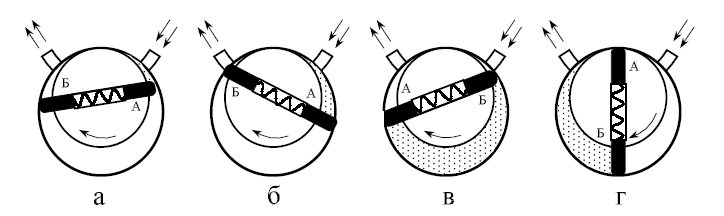
\includegraphics[width=0.9\linewidth]{Устройство фв насоса.PNG}
	\caption[]{Схема действия ротационного двухпластинчатого форвакуумного насоса}
	\label{fig:Схема ФВ насоса}
\end{figure}
Устройство и принцип действия \textit{диффузионного насоса} схематически изображены на рис 2. Такой насос работает в тысячи раз быстрее форвакуумного. Его действие основано на диффузии. Масло, налитое в сосуд А, подогревается электрической печкой. Пары масла поднимаются по трубке Б и вырываются из сопла В. Струя паров увлекает молекулы газа, которые поступают из откачиваемого сосуда через трубку ВВ. В трубке Г мало осаждается и стекает вниз. Оставшийся газ, выходя в трубку ФВ, откачивается форвакуумным насосом. \\
Диффузионный насос работает наиболее эффективно, когда длина свободного пробега молекул примерно равна ширине кольцевого зазора между соплом В и стенками трубки ВВ. Давление насыщенных паров масла при рабочей температуре, создаваемой обогревателем сосуда А, много больше $5\cdot 10^{-2}$ торр, поэтому пары масла создают плотную струю, увлекающую с собой молекулы газа.
\begin{figure}[!h]
	\centering
	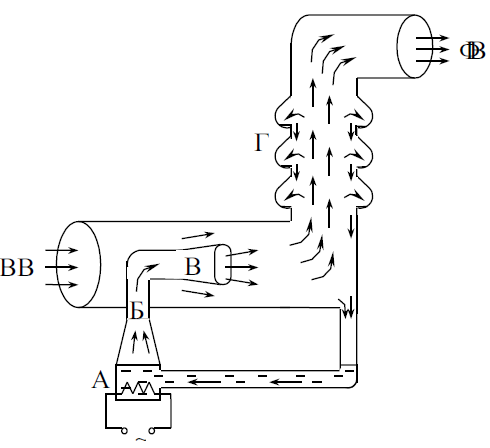
\includegraphics[width=0.4\linewidth]{Устройство вв насоса.PNG}
	\caption[]{Схема работы диффузионного насоса}
	\label{fig:Схема ВВ насоса}
\end{figure}
 Диффузионный насос, используемый в нашей установке (см. рис 1) имеет две ступени и соответственно два сопла. Одно сопло вертикальное (первая ступень), второе горизонтальное (вторая ступень). За второй ступенью имеется ещё одна печь, но пар из этой печи поступает не в сопло, а по тонкой трубке подводится ближе к печке первой ступени. Эта печь осуществляет фракционирование масла. Легколетучие фракции масла, испаряясь, поступают в первую ступень, обогащая её. По этой причине плотность струи первой ступени выше, и эта ступень начинает откачивать при более высоком давлении в форвакуумной части. Вторая ступень обогащается малолетучими фракциями масла. Плотность струи второй ступени меньше, но меньше и давление насыщенных паров. Соответственно, в откачиваемый объем поступает меньше паров масла, и его удаётся откачать до более высокого вакуума.  \\
 \begin{figure}[H]
 	\begin{center}
 		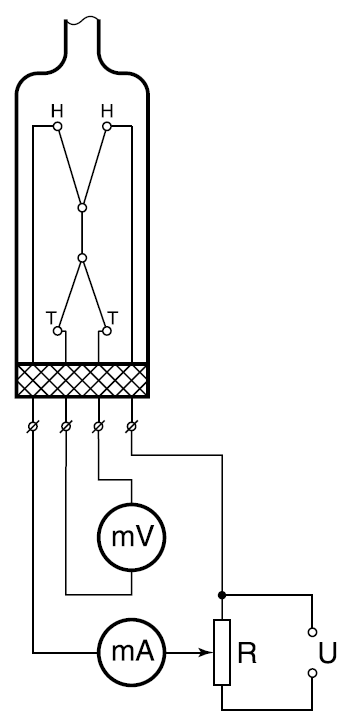
\includegraphics[width=0.5\linewidth]{термопара.PNG}
 		\caption{Схема термопарного манометра с лампой ЛТ-2}
 		\label{fig:Схема термопары}
 	\end{center}
 \end{figure}
 \textit{Термопарный манометр.} Чувствительным элементом манометра является платиново-родиевая термопара, спаянная с никелевой нитью накала и заключённая в стеклянный баллон. Устройство термопары пояснено на рис. 4. По нити накала НН пропускается ток постоянной величины. Для установки тока служит потенциометр R, расположенный на передней панели вакуумметра. Термопара ТТ присоединяется к милливольтметру, показания которого определяются температурой нити накала и зависят от отдачи тепла в окружающее пространство. \\
 Потери тепла определяются теплопроводностью нити и термопары, теплопроводностью газа, переносом тепла конвективными потоками газа внутри лампы, и теплоизлучением нити (инфракрасное тепловое излучение). В обычном режиме лампы основную роль играет теплопроводность газа. При давлениях, не меньших 1 торр, теплопроводность газа, а вместе с ней и ЭДС термопары практически не зависят от давления газа, и прибор не работает. \\
 При улучшении вакуума средний свободный пробег молекул становится сравнимым с диаметром нити, теплоотвод падает, и температура спая возрастает. При вакууме порядка $10^{-3}$ торр теплоотвод, осуществляемый газом, становится сравнимым с другими потерями тепла, и температура становится практически постоянной. Градуировочная кривая термопары приведена на рис. 5. \\
 \begin{figure}[!h]
 	\centering
 	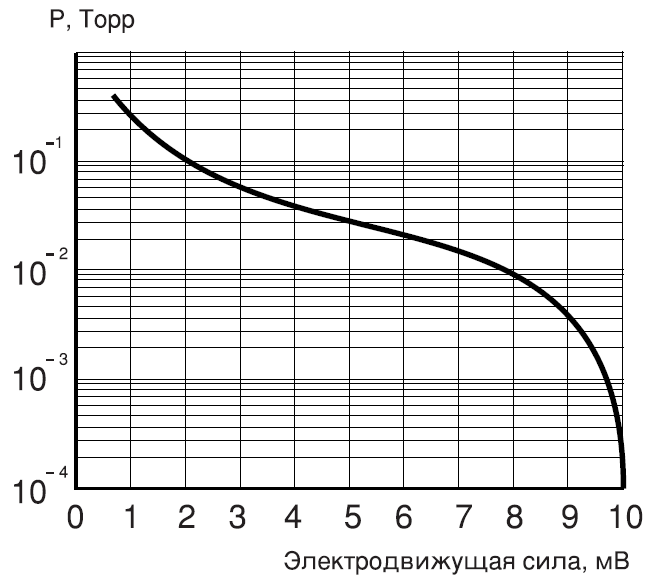
\includegraphics[width=0.4\linewidth]{градуировочная кривая.PNG}
 	\caption[]{Градуировочная кривая термопары ЛТ-2}
 	\label{fig:Градуировочная кривая}
 \end{figure}
 \begin{figure}[H] %если не лезет, но с новой стр
	\begin{center}
		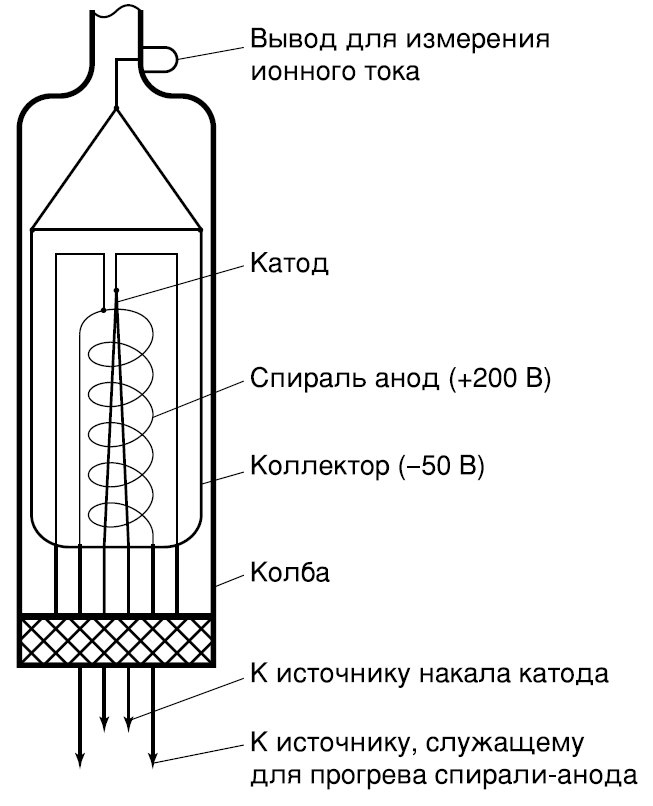
\includegraphics[width=0.4\linewidth]{лампа.PNG}
		\caption{Схема ионизационной лампы ЛТ-2}
		\label{fig:лампа}
	\end{center}
\end{figure}
\textit{Ионизационный манометр.} Схема ионизационного манометра изображения на рисунке 6. Он представляет собой трехэлектродную лампу. Электроны испускаются раскалённым катодом и увлекаются электрическим полем к аноду, имеющему вид редкой спирали. Проскакивая за её витки, электроны замедляются полем коллектора и возвращаются к аноду. Прежде чем осесть на аноде, они успевают много раз пересечь пространство между катодом и коллектором. На своём пути электроны ионизуют молекулы газа. Ионы, образовавшиеся между анодом и коллектором, притягиваются полем коллектора и определяют его ток. \\
  Накалённый катод ионизационного манометра перегорает, если давление в системе превышает $10^{-3}$ торр, поэтому перед его включением необходимо проверить давление термопарным манометром. \\
 \subsection*{Процесс откачки}
Опишем процесс откачки математически: 
Пусть W --- объем газа, удаляемого из сосуда при данном давлении за единицу времени, $Q_i$ для различных значений i обозначим различные притоки газа в сосуд (в единицах PV), такие как течи извне $Q_\text{и}$, десорбция с поверхностей внутри сосуда $Q_\text{д}$, обратный ток через насос $Q_\text{н}$. Тогда, приравнивая убыль газа из сосуда (с точностью до $RT/\mu$) в единицу времени $-VdP$ и сумму перечисленных токов? имеем:
 \begin{equation}
 	-VdP = (PW - \sum_i Q_i)dt
 \end{equation}
 При достижении предельного вакуума устанавливается давление $P_{\text{пр}}$, и $dP = 0$. Тогда
 \begin{equation}
 	 W = ( \sum_i Q_i )/P_{\text{пр}}
 \end{equation}
 Поскольку обычно $Q_\text{и}$ постоянно, а $Q_\text{н}$ и $Q_\text{д}$ слабо зависят от времени, также считая постоянной W, можем проинтегрировать (1) и получить:
 \begin{equation}
 	P - P_{\text{пр}} = (P_0 - P_{\text{пр}})\exp(-\frac{W}{V}t)
 \end{equation}
Полная скорость откачки $W$, собственная скорость откачки насоса $W_{\text{н}}$ и проводимости элементов системы $C_1, C_2,...$ соотносятся согласно формуле (4), и это учтено в конструкции установки.
 \begin{equation}
 \frac{1}{W} = \frac{1}{W} + \frac{1}{C_1} + \frac{1}{C_2} + ...
\end{equation}

\subsection*{Течение газа через трубу}
Характер течения газа существенно зависит от соотношения между размерами системы и длиной свободного пробега молекул. При атмосферном и форвакуумном давлениях  длина свободного пробега меньше диаметра трубок, и течение газа определяется его вязкостью, т.е. взаимодействием молекул. При высоком вакууме течение существеннее определяется взаимодействием со стенками \\
Для количества газа, протекающего через трубу длины $l$ и радиуса $r$ в условиях высокого вакуума, справедлива формула:
\begin{equation}
	\frac{d(PV)}{dt} = \frac{4}{3}r^3\sqrt{\frac{2\pi RT}{\mu}}\frac{P_2 - P_1}{l}
\end{equation}
Если труба соединяет насос установку, то давлением $P_1$ у насоса можно пренебречь. Давление в сосуде $P = P_2$. Тогда имеем:
\begin{equation}
C_\text{тр} = \left(\frac{dV}{dt}\right)_\text{тр} = \frac{4r^3}{3l}\sqrt{\frac{2\pi RT}{\mu}}
\end{equation}
Для пропускной способности отверстий имеется формула
\begin{equation}
C_\text{отв} = \left(\frac{dV}{dt}\right)_\text{отв} = S\frac{\bar{\upsilon}}{4}
\end{equation}
Для воздуха при комнатной температуре $\bar{\upsilon}/4 = 110~\text{м/с} = 11~\text{л/c}\cdot\text{см}^2$.


\section{Результаты и их обсуждение}
Согласно методичке измерены объёмы форвакуумной и высоковакуумной части установки (Прил. \ref{app_1}). Полученные объёмы соответственно 
равны $V_1 = &V_1&$ $\text{м}^3$ и $V_2 = &V_2&$ $\text{м}^3$. С использованием диффузионного насоса 
получен высокий вакуум в высоковакуумной части установки. После этого было произведение отключение насоса от системы 
и измерена зависимость давления в установке от времени. После произведено повторное подключение насоса к системе 
и измерена зависимость давления в установке от времени (Рис. \ref{fig:Pt}). 

\begin{figure}[H]
    \centering
    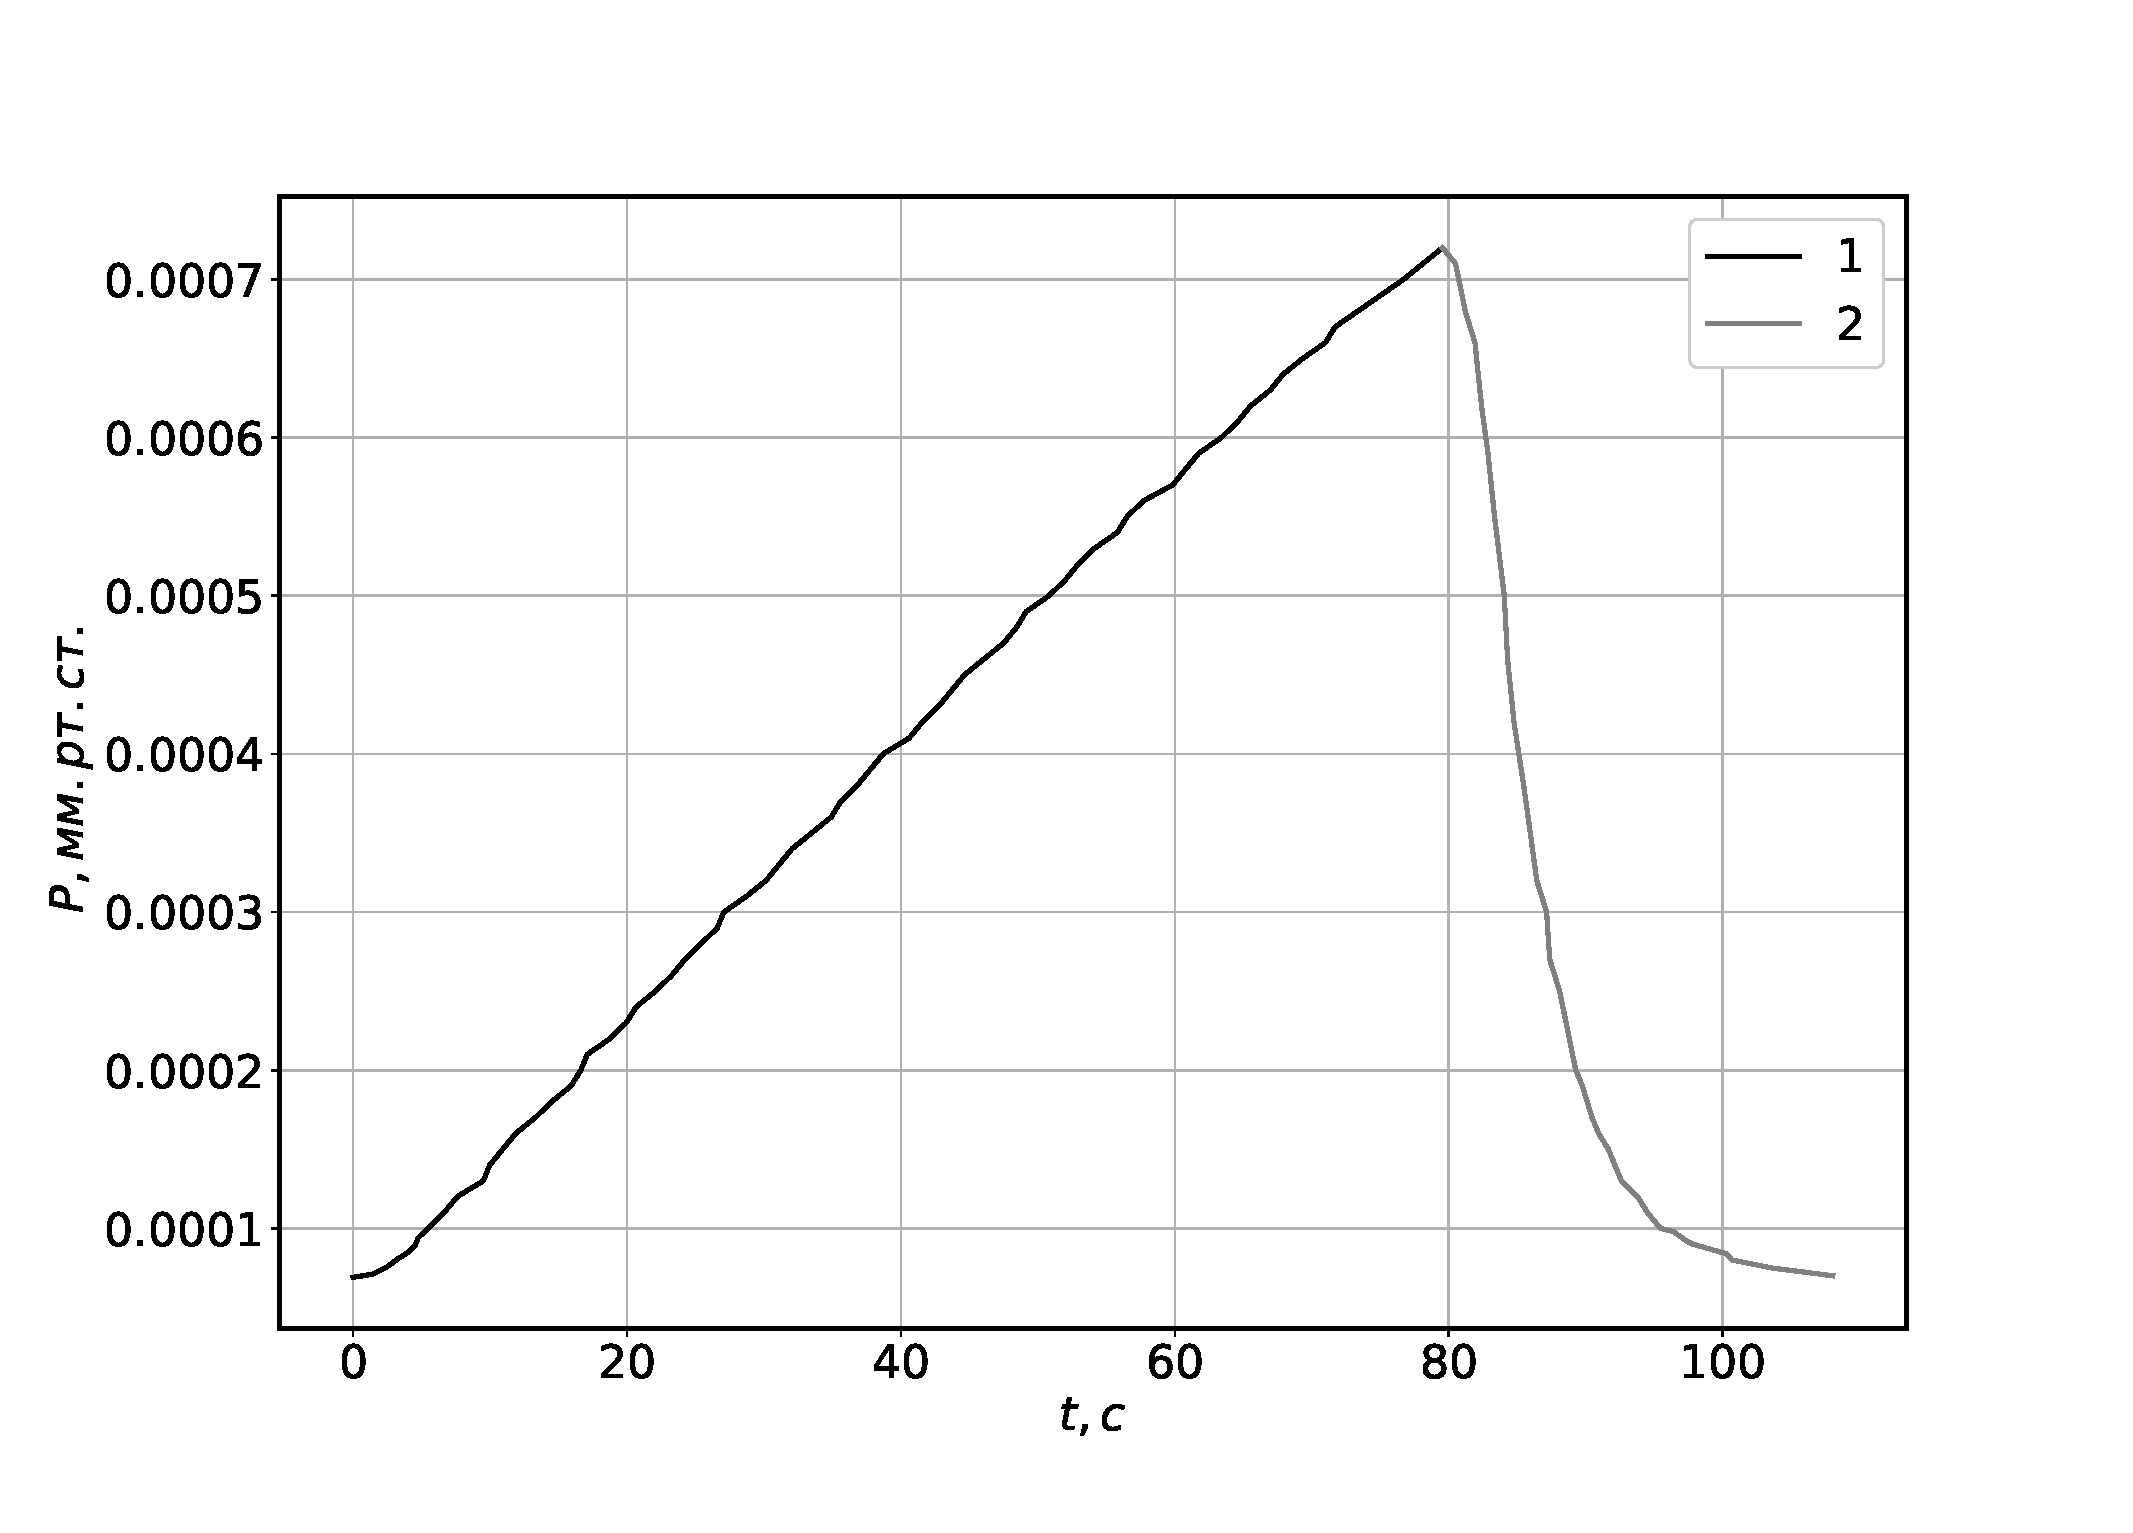
\includegraphics[width=0.8\textwidth]{Pt.eps}
    \caption{Зависимость давления $P$, измеренного на ионизационном манометре в зависимости от 
    времени $t$ при выключенной откачке (линия 1), и при включенном диффузионном насосе (линия 2).}
    \label{fig:Pt}
\end{figure}

Согласно теории, участок 2 на графике соответсвует экспоненциальному уменьшению давления, поэтому перестроим 
данную часть графика в логарифмическом масштабе (Рис. \ref{fig:Pdownt}). По графику видно, что полученная 
зависимость является линейной, что подтверждает корректность используемой модели. В таком случае возможно 
вычислить скорость откачки $W$: 
\[
    W = - V_2 b, 
\] 
где $b$ - коэффициент наклона графика в логарифмическом масштабе. В таком случае $W = &W1&$ $\frac{\text{м}^3}{\text{с}}$.     
\begin{figure}[H]
    \centering
    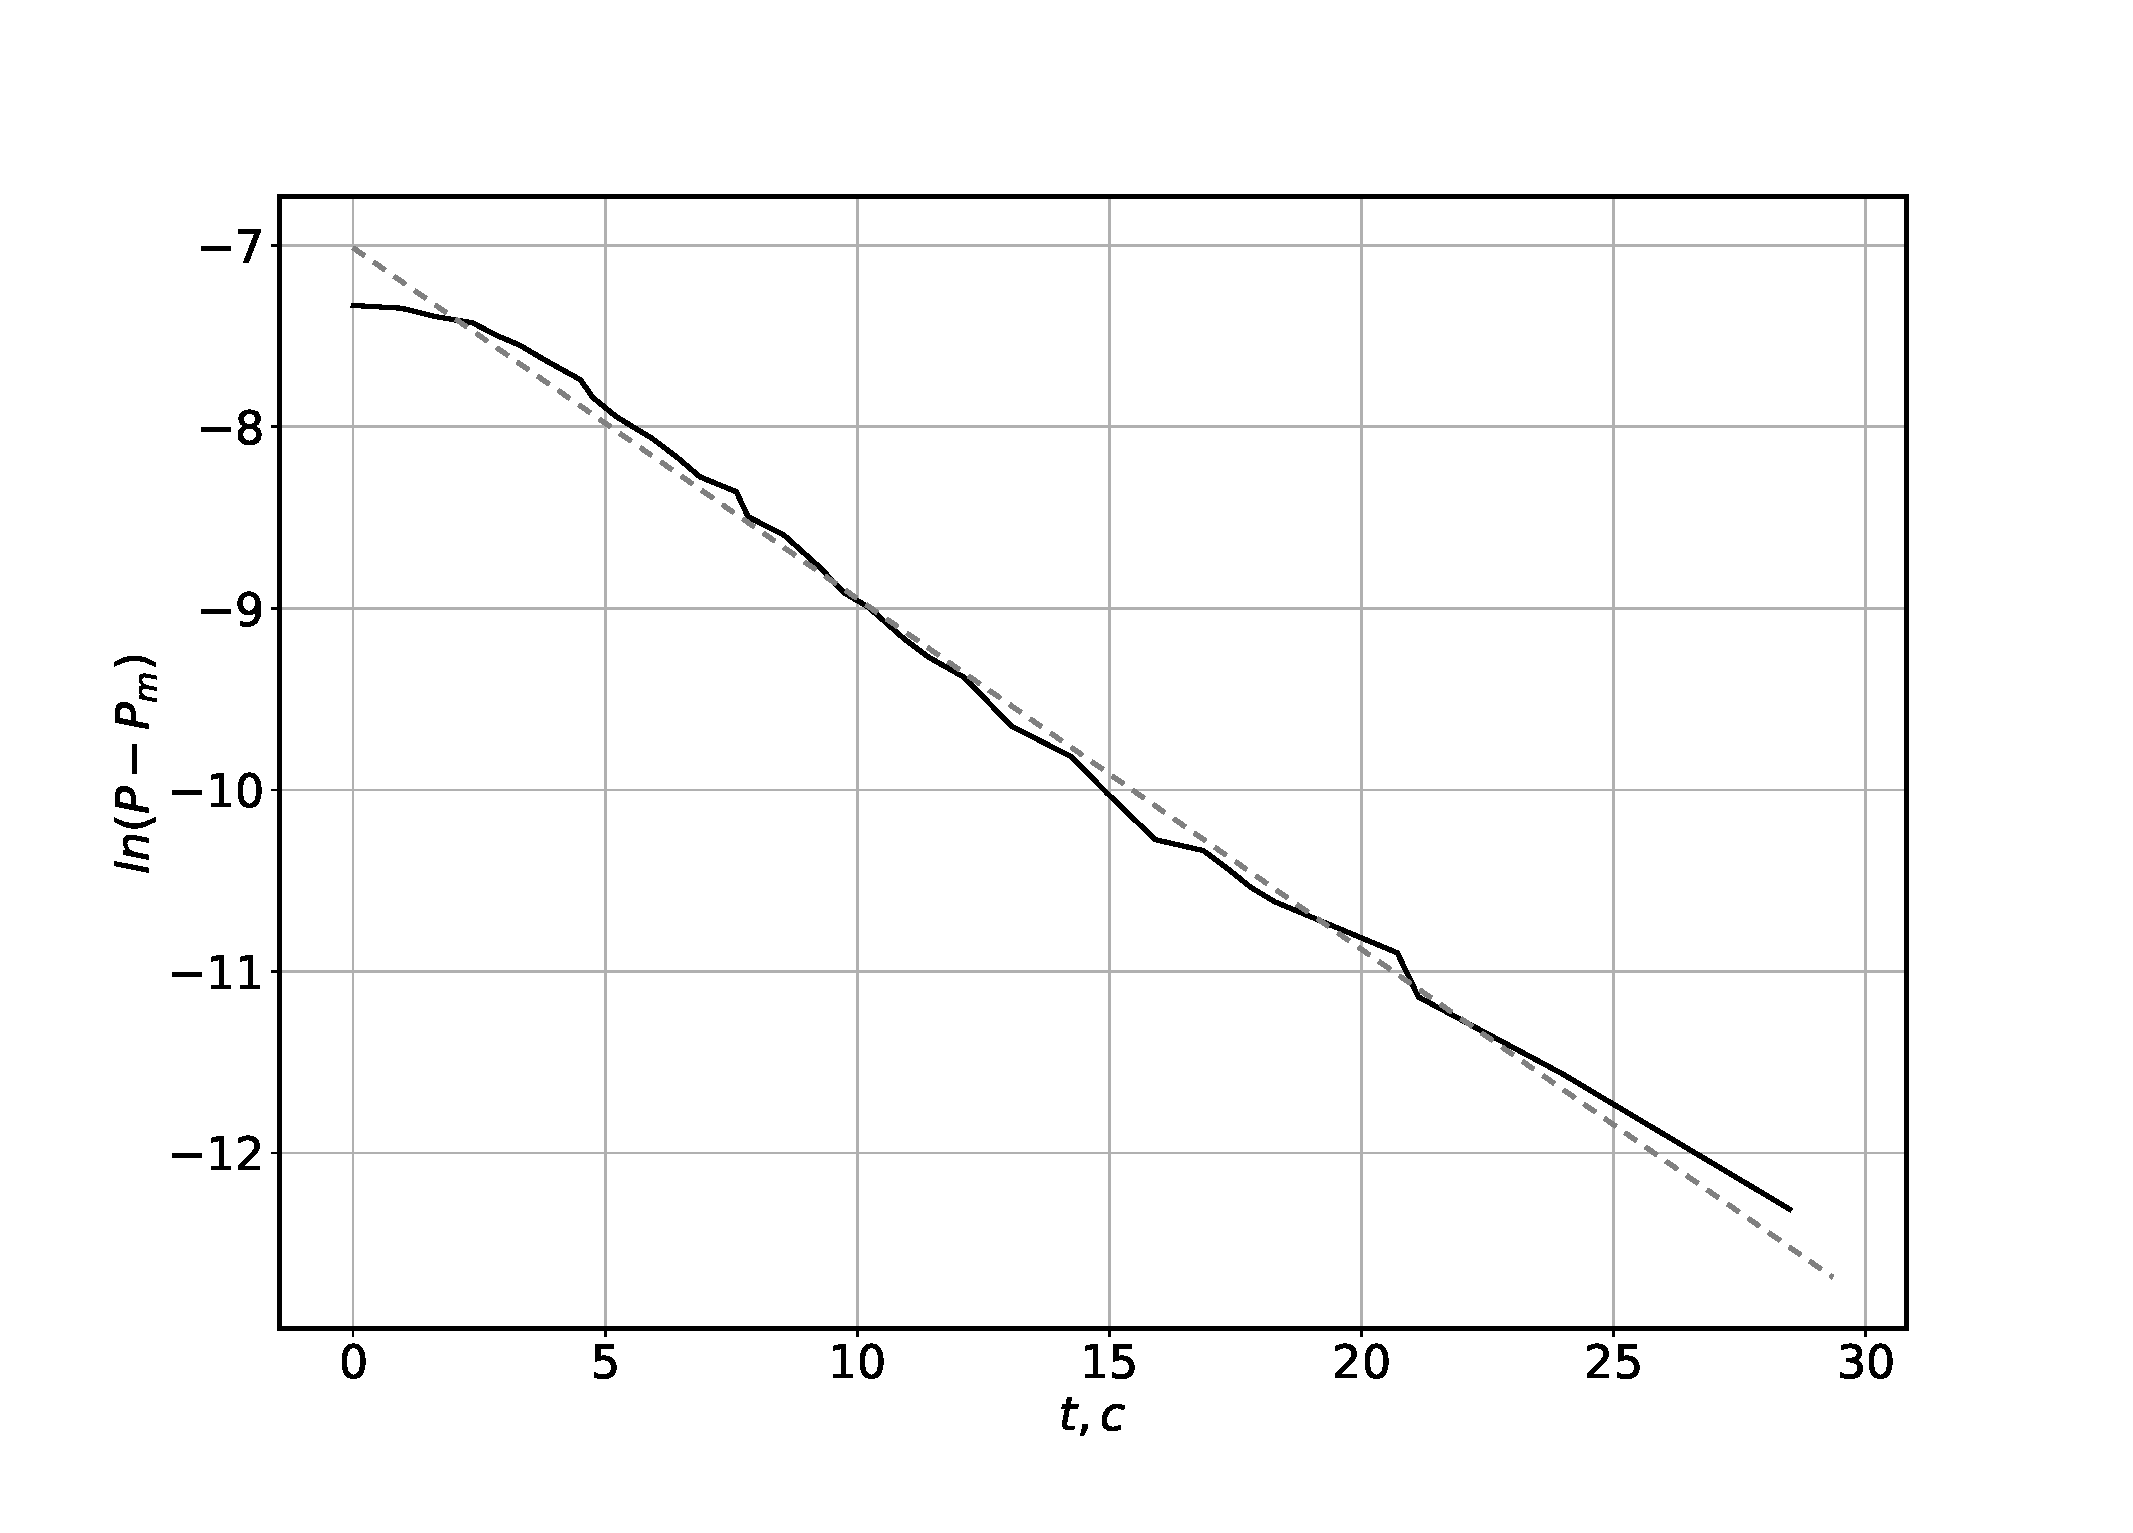
\includegraphics[width=0.8\textwidth]{Pdownt.eps}
    \caption{Зависимости давления $P$ в установке от времени $t$ при включенном насосе.}
    \label{fig:Pdownt}
\end{figure}

Для того чтобы найти количество газа, выходящее из системы из-за микротечей, построим график зависимости 
давления в системе от времени при отключенном насосе (Рис. \ref{fig:Pupt}). 

\begin{figure}[H]
    \centering
    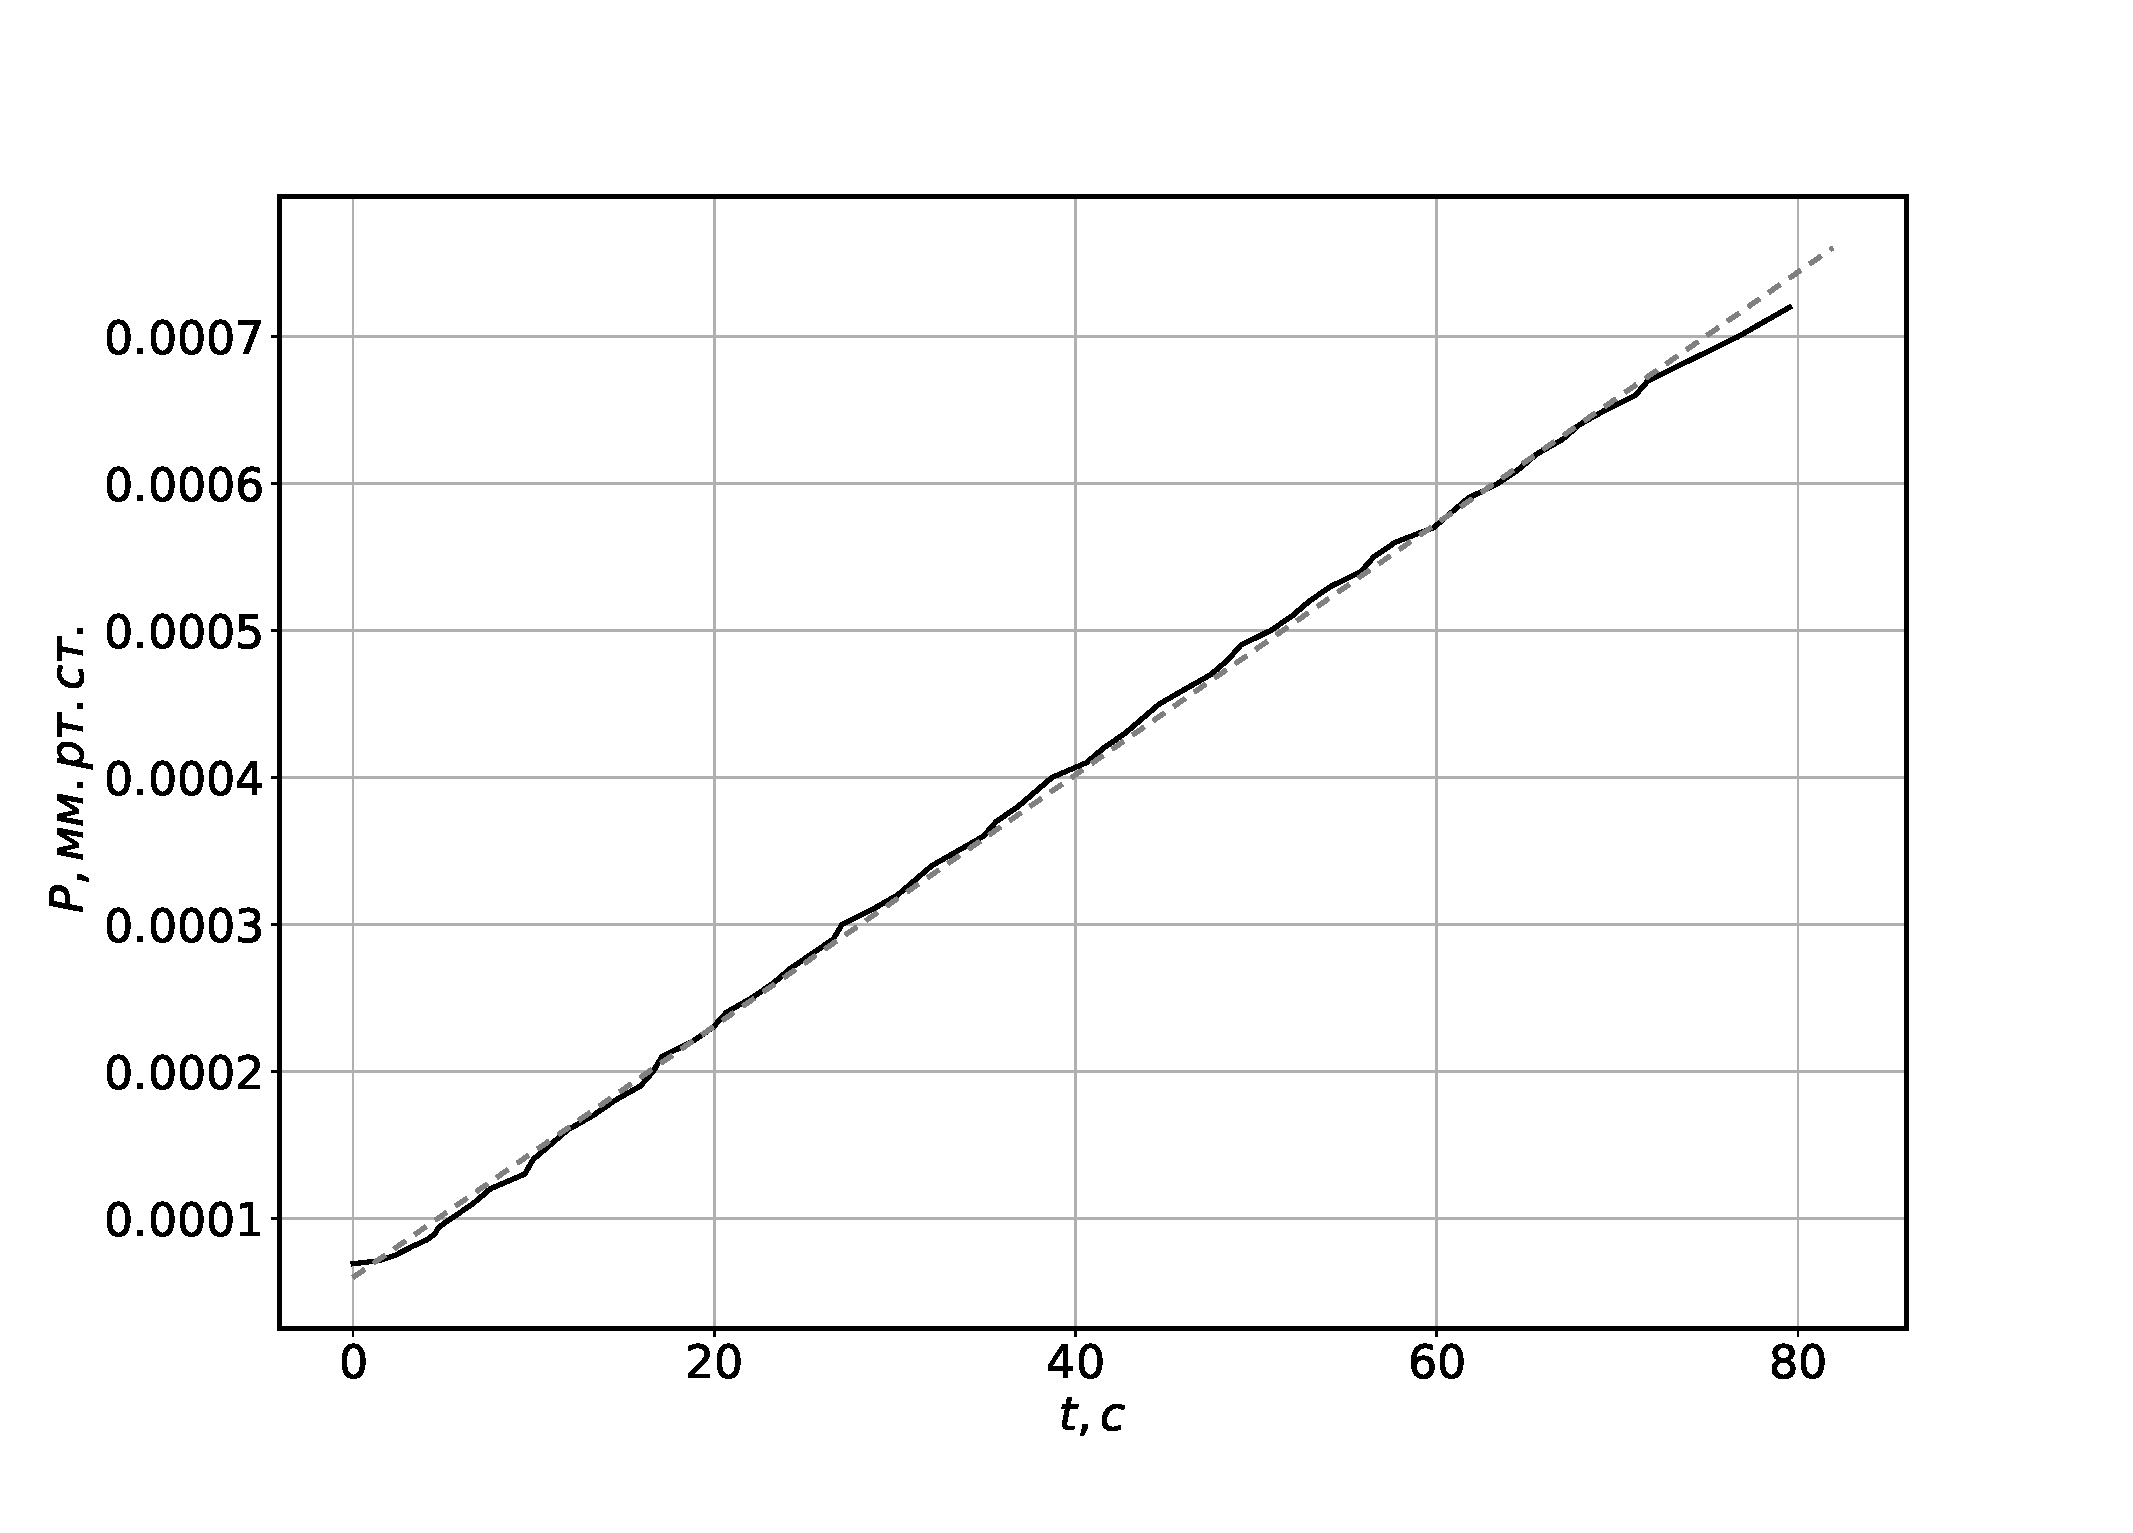
\includegraphics[width=0.8\textwidth]{Pupt.eps}
    \caption{Зависимости давления $P$ в установке от времени $t$ при выключенном насосе.}
    \label{fig:Pupt}
\end{figure}

Полученный график хорошо аппроксимируется прямой, что подтверждается теоретической моделью, 
в таком случае считая, что уменьшение давления характеризуется только утечкой через микрощели, имеем формулу: 
\[
    Q = b V_2,
\]
где $b$ - коэффициент наклона. Полученное значение величины утечки равна 
$Q = &Q&$ $\text{(мм. рт. ст)} \frac{\text{м}^3}{\text{с}}$.    

Далее в систему была введена искусственная течь и измерено установившееся давления $P_y = &Py&$ $\text{мм. рт. ст}$. 
Тогда возможно расчитать мощность откачки как 
\[
    W = \frac{1}{P_y - P_m} \frac{4}{3} \frac{d}{2}^3 \sqrt{\frac{2\pi RT}{\mu}} \frac{P_v}{L}, 
\]  
где $P_v$ - давление в форвакуумной части установки, $P_y$ - установившееся давление, $P_m$ - 
минимальное значение откачки. В таком случае $W = &W2&$ $\frac{\text{м}^3}{\text{с}}$. 
Полученное значение отличается в несколько раз от полученного по графику. Такое расхождение 
можно объяснить тем, что на представленной установке установлен мощный насос, из-за 
чего характерное время установления $P_y$ велико, что может давать большую погрешность измерения 
$P_y$.      

\section{Выводы}
Получен ваккум с давлением $P = &Pm&$ $\text{мм. рт. ст.}$. Измерена мощность откачки насоса а также 
величина микротечей утсановки.  

\section{Использованная литература}
\begin{thebibliography}{9}
    \bibitem{LabBook}
    Лабораторный практикум по общей физике, Том 1, под редакцией А. Д. Гладуна
    \bibitem{Kirichenko}
    Н.А. Кириченко «Термодинамика, статистическая и молекулярная физика».
\end{thebibliography}

\section{Приложения}
\subsection{Параметры установки и погрешности приборов} \label{app_1}
\end{document}